%
% Sección de BPS.
% Artículo.
% Proyecto Lovelace.
%

\subsection{BPS}

% Borrador de la sección de BPS (v2)

Algoritmo de cifrado que preserva el formato capaz de cifrar cadenas formadas
por cualquier conjunto de caracteres, descrito en \cite{bps} y cuyo nombre
proviene de las iniciales de los apellidos de sus autores Eric Brier, Thomas
Peyrin y Jacques Stern, aunque en el estándar \cite{nist_fpe}, el NIST lo
nombra como FF3.

BPS se conforma de 2 partes: un cifrado interno $BC$ que se encarga de cifrar
bloques de longitud fija, usando a su vez un cifrado por bloques $F$; y un modo
de operación especial, encargado de extender la funcionalidad de $BC$ y permitir
cifrar cadenas de un longitud de hasta $max_b \cdot 2^{16}$ caracteres, donde
$max_b$ es la longitud máxima que puede tener una cadena para cifrarse con $BC$.

Este cifrado interno utiliza una red Feistel alternante y se define como
$BC_{F,s,b,w}(X,K,T)$, donde: $F$ es un cifrado por bloques con $f$ bits de
salida, como puede ser TDES o AES; $s$ es la cardinalidad del alfabeto de la
cadena a cifrar, $b$ es su longitud, $w$ es el número de rondas de la red
Feistel, $X$ es la cadena, $K$ es una llave acorde al cifrado $F$, y $T$ es
un \textit{tweak} de 64 bits.

El funcionamiento del cifrado $BC$ es descrito en la figura \ref{proceso_bc}.

\begin{figure}
  \begin{center}
    \begin{tabular}{|l|}
      \hline
      \begin{minipage}{0.5\textwidth}
        \begin{tabbing}
          \ \ \ \ \ \=\ \ \ \ \=\ \ \ \ \=\ \ \ \ \=\ \ \ \ \=\ \ \ \ \=\ \ \
          \ \kill \\
          \ \ \ \ {\bf Algoritmo} Cifrado $BC_{F,s,b,w}$($X$,$K$,$T$)\\
          \>  1. \> $T_R\: \gets\: T\: \mod\: 2^{32}$ y 
                    $T_L\: \gets\: (T\: -\: T_R) / 2^{32}$ \\
          \>  2. \> $l \gets \lceil b/2 \rceil$ \\
          \>  3. \> $r \gets \lfloor b/2 \rfloor$ \\
          \>  4. \> $L_0\: \gets\: \sum_{j=0}^{l-1}\: X[j] \cdot s^j$ \\
          \>  5. \> $R_0\: \gets\: \sum_{j=0}^{r-1}\: X[j+l] \cdot s^j$ \\
          \>  6. \> {\bf para} $i=0$ {\bf hasta} $i=w-1$: \\
          \>  7. \> \> {\bf si} $i$ es par: \\
          \>  8. \> \> \> $L_{i+1}\: \gets\: L_i\: \boxplus\: F_K((T_R \oplus i)
                          \cdot 2^{f-32}\: +\: R_i)\quad (mod\ s^l)$ \ \ \ \ \\
          \>  9. \> \> \> $R_{i+1}\: \gets\: R_i$ \\
          \> 10. \> \> {\bf si} $i$ es impar: \\
          \> 11. \> \> \> $R_{i+1}\: \gets\: R_i\: \boxplus\: F_K((T_L \oplus i)
                          \cdot 2^{f-32}\: +\: L_i)\quad (mod\ s^r)$ \ \ \ \ \\
          \> 12. \> \> \> $L_{i+1}\: \gets\: L_i$ \\
          \> 13. \> {\bf para} $i=0$ {\bf hasta} $i=l-1$: \\
          \> 14. \> \> $Y_L[i] \gets L_w\ mod\ s$ \\
          \> 15. \> \> $L_w \gets (L_w - Y_L[i])/s$ \\
          \> 16. \> {\bf para} $i=l$ {\bf hasta} $i=r-1$: \\
          \> 17. \> \> $Y_R[i] \gets R_w\ mod\ s$ \\
          \> 18. \> \> $R_w \gets (R_w - Y_R[i])/s$ \\
          \> 19. \> $Y \gets Y_L \parallel Y_R$ \\
        \end{tabbing}
        \end{minipage}\\
        \hline
      \end{tabular}
    \end{center}
    \caption{\label{proceso_bc} Cifrado interno BC.}
\end{figure}

Para cada bloque a cifrar, el cifrado $BC$ debe instanciarse con una longitud
de $max_b = 2 \cdot log_s(2^{f-32})$ caracteres, y cuando la longitud total
del mensaje a cifrar no sea múltiplo de este valor, en el último bloque $BC$
se tendrá que instanciar con una longitud igual a la de ese bloque.

El modo de operación de BPS es un variación de CBC, con la diferencia de que
usa sumas modulares carácter por carácter en lugar de aplicar operaciones
\textit{xor}, además de que no emplea un vector de inicialización.

Otra característica de este modo de operación es que utiliza un contador $u$
para aplicar un \textit{xor} a los 16 bits más significativos de cada mitad
del \textit{tweak} $T$ que utiliza BPS, por lo cual este se puede ver como
una función $u(n) = n \cdot (2^{16} + 2^{48})$.

El funcionamiento del modo de operación se describe en la figura \ref{modo_bps}.

\begin{figure}
  \begin{center}
    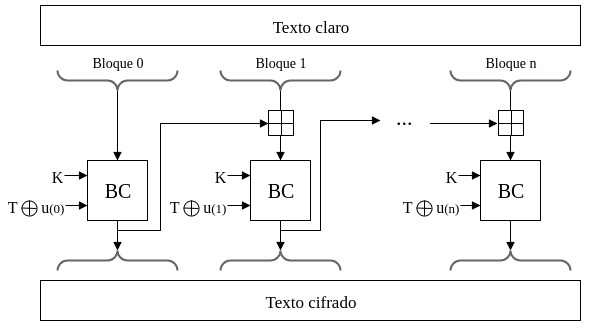
\includegraphics[width=0.85\linewidth]
    {../../../diagramas_comunes/bps/modo_de_operacion_bps}
    \caption{Modo de operación de BPS.}
    \label{modo_bps}
   \end{center}
\end{figure}

El PCI clasifica a este algoritmo dentro de los método de de generación de
tokens reversibles criptográficos, pero desde el punto de vista de este
trabajo se tiene que es un método criptográfico reversible.

